\chapter{Introduction}
According to the Reuters Institute, 36\% of French adults use social media as a source of news.\footnote{\url{http://media.digitalnewsreport.org/wp-content/uploads/2018/06/digital-news-report-2018.pdf?x89475}}  This share has declined since 2017, but this is mostly due to a decrease in the use of Facebook, while other networks are stable (like Twitter) or growing rapidly. This evolution of news consumption may reflect a growing interest for stories that are usually not covered by traditional news media, or that are covered in a different way. This raises the question of the type of news that is mostly shared on social networks: are the citizens differently informed when they use social network as a gateway to news? 
\newline

In response to the transformation of news consumption, one should expect a change in the production of news by traditional media outlets. \citet{mcgregor_twitter_2018} find that journalists using Twitter as part of their daily work consider tweets as newsworthy as headlines from the Associated Press. Does this change in the perception of journalists has an effect on the type of stories they choose to report? Does the success of a story on social media impacts the news production by traditional news media outlets?
\newline

The objective of this thesis is to investigate the role of Twitter in the evolution of both news consumption and news production in recent years. We aim at understanding what kind of news are  amplified by the sphere of social networks, and, conversely, to show in which cases events born on the social networks become a subject relayed by traditional media outlets. The challenge is to quantify and analyze precisely the relationships between the two spheres, in a context of very strong influence of each sphere on the other. 
\newline

Indeed, stories do not spread only in one direction, from news media to social networks or from social networks to news media. The recent Benalla case in France can be used as an illustration of the different rebounds that an event can have in both spheres: videos of Alexandre Benalla wearing a police helmet and hitting a protester where published on social media on May 1, 2018. However, he was only identified as an aide from President Macron's office on July 18, by the newspaper \textit{Le Monde}. After this first article, traditional media outlets started to investigate on the missions of Mr. Benalla. Both journalists and Twitter users published numerous pictures of Alexandre Benalla in official appearances of the President, including during the period when he was allegedly suspended. The newspaper ``Sud Ouest" used the term ``photo hunt" to qualify the attitude of social media users and photo reporters\footnote{\url{https://www.sudouest.fr/2018/07/23/affaire-benalla-quand-les-reseaux-sociaux-s-amusent-5256018-10458.php}}. On July 30, a Belgian organization called DisinfoLab evoked an artificial swelling of the number of messages on Twitter related to the Benalla case.\footnote{\url{https://twitter.com/DisinfoEU/status/1023903729668575242}} In the partial results published on that day, the ``overactivity" of some Twitter accounts and ``pro-Russian" accounts were mentioned. On August 8, DisinfoLab published the entire study,\footnote{\url{https://spark.adobe.com/page/Sa85zpU5Chi1a/}} showing no evidence that an organized Russian intervention has sought to amplify the Benalla case on Twitter. However, several media outlets had already relayed the (wrong) information that ``Russian bots"  had influenced the reaction of the public on Twitter.\footnote{\url{https://abonnes.lemonde.fr/les-decodeurs/article/2018/08/08/l-impossible-quete-des-bots-russes-de-l-affaire-benalla_5340540_4355770.html?}}
\newline

%%%%%%%%%%%%%%%%%%%%%%%%
\begin{figure}
\begin{center}
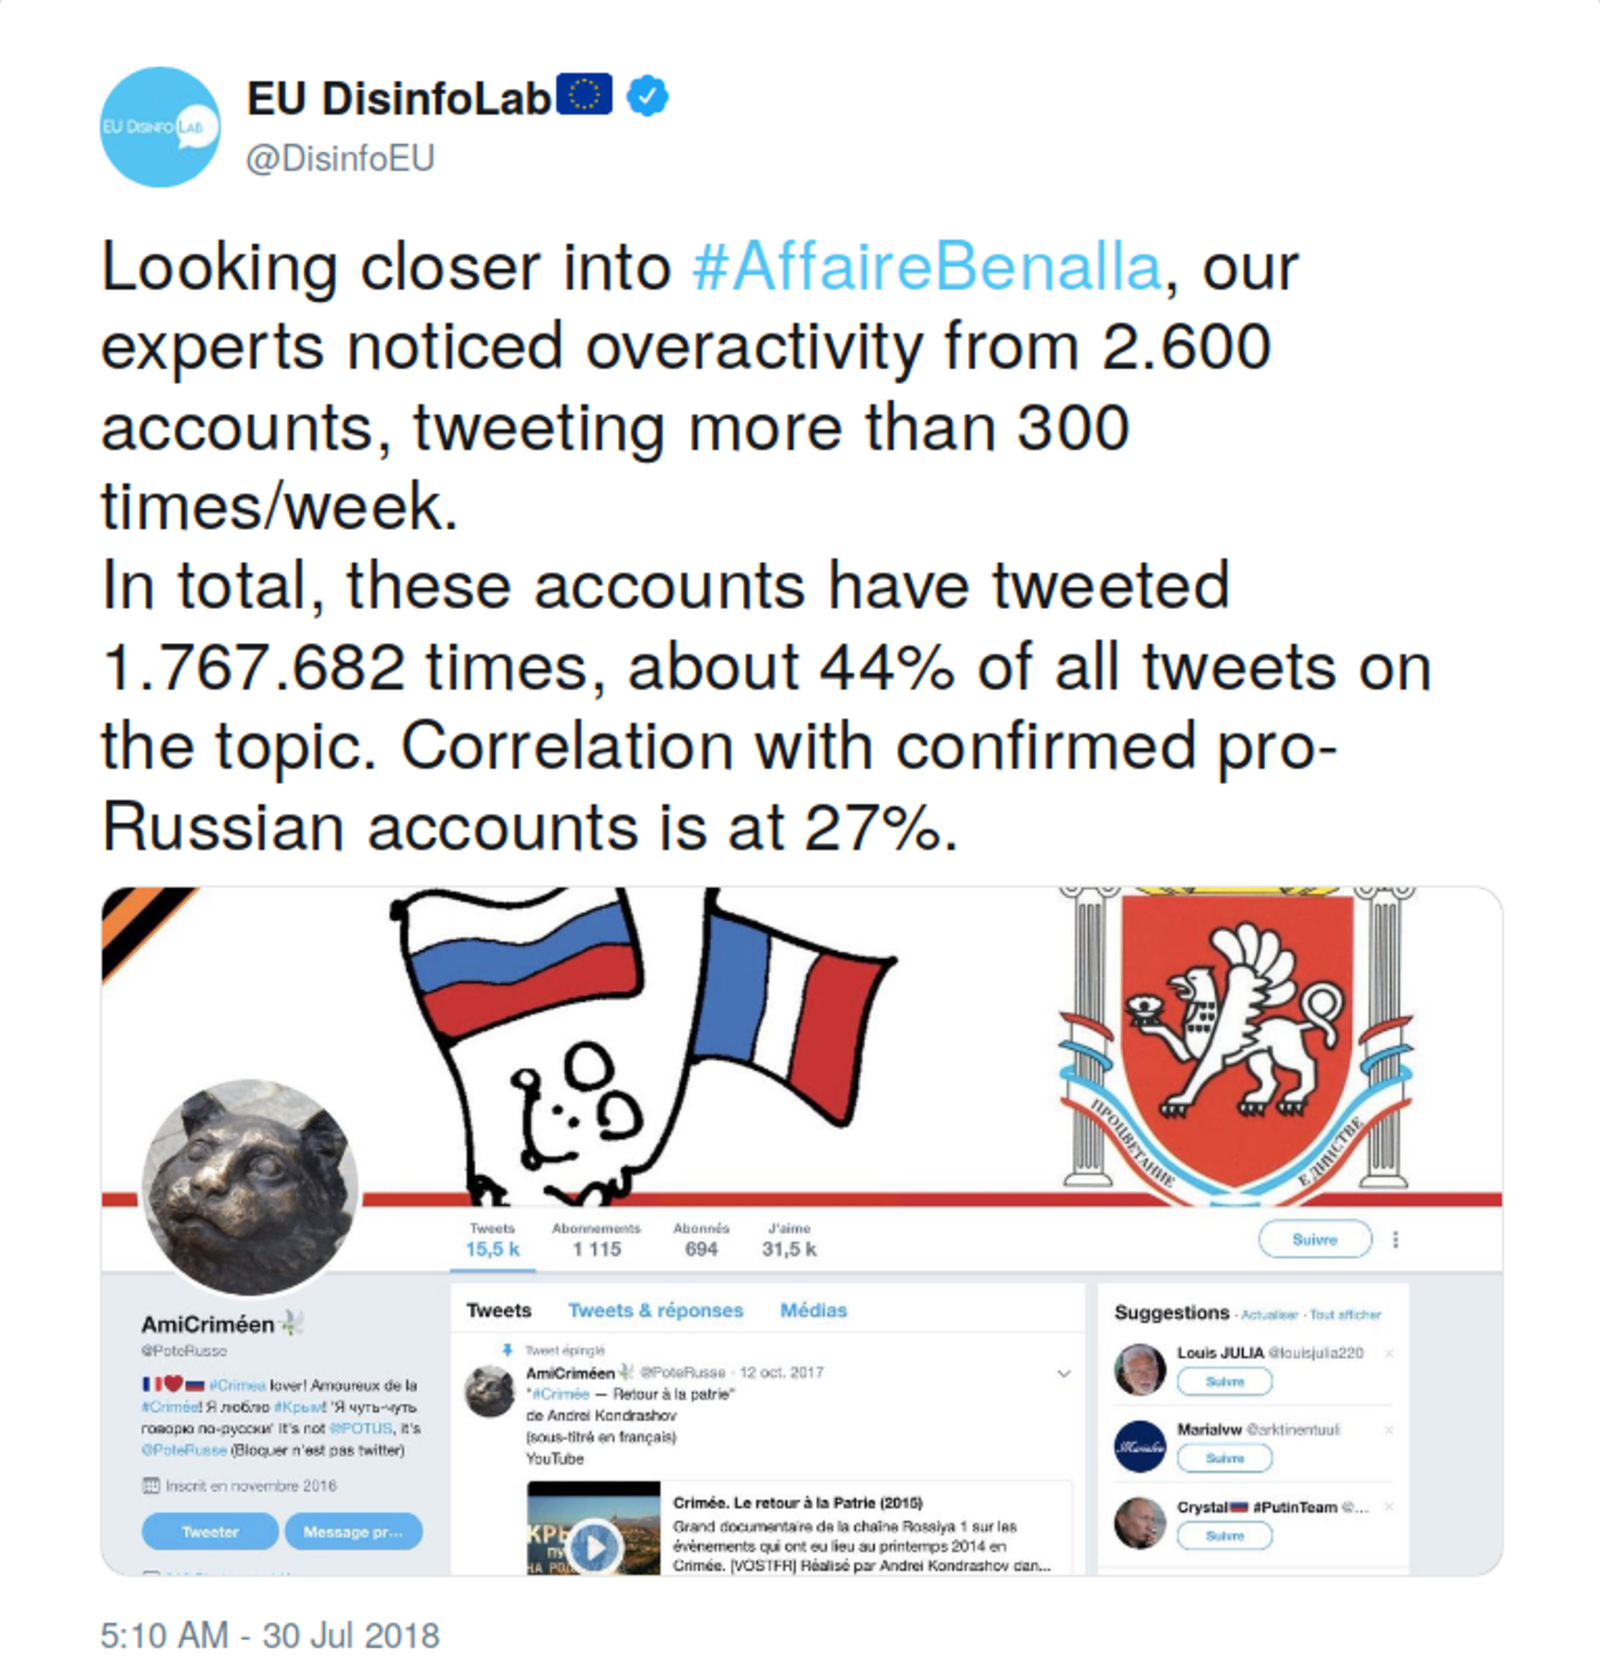
\includegraphics[scale=.35]{images/Screenshot_DisinfoLab_AffaireBenalla.pdf}
\end{center}
{\scriptsize \textbf{Notes:} These preliminary results were nuanced in the full study published on August 8, 2018}
\caption{Tweet from DisinfoLab, an organization working on disinformation, about the ``overactivity" of some Twitter accounts during the Benalla scandal}
\label{Figure:DisinfoLab}
\end{figure}
%%%%%%%%%%%%%%%%%%%%%%%%

This is only one example of the plurality of ``interaction patterns" \citep{ning_uncovering_2015} between social networks and traditional media that can occur in the news agenda. Here, social networks are first used as a source by news outlets (most videos of Alexandre Benalla used by journalists where initially published on Twitter by witnesses of the May 1 demonstration). Then, they participate to the controversy raised by traditional media outlets and amplify it. Finally, the amplitude of the echo on Twitter is discussed by media outlets. Other types of interaction patterns exist, for example ``break on Twitter first" stories (like the hashtag \#MakeOurPlanetGreatAgain posted on June 2017 by Emmanuel Macron that was widely commented by traditional news media) or Twitter movements that criticize traditional media (for example, Twitter users reacted to the shocking images of victims of the Nice attack with the hashtag \#CSACoupezTout, which led the \textit{France Télévisions} group to apologize\footnote{\url{https://www.francetvinfo.fr/economie/medias/france-televisions/edition-speciale-sur-l-attentat-de-nice-france-televisions-presente-ses-excuses_1548057.html}}). We aim at developing measurement tools and analysis criteria to characterize and quantify these interaction patterns.
\newline

The originality of this project is its bi-disciplinary nature. On the one hand, it will consist of an analysis in media economics, in order to determine the factors that influence the relative impact of a story on Twitter and in traditional news media. This thesis will have to take into account several types of measures of the media impact, both absolutely (number of tweets, number of articles), but also related to the membership networks of the users emitting the information:  a story spreads more widely if it is issued within a majority group \citep{HalberstamKnight2016}, and information is more easily relayed if it emanates from the account of a journalist or a politician \citep{harder_making_2016}. On the other hand, it will require advanced computer science research to design novel approaches to Twitter event detection and clustering, using both Natural Language Processing and Image Processing.
\newline

\section{Choice of Twitter}


\section{Choice of France}


\section{Characterization of events}


\section{Detailed Outline}